\chapter{The Rename Stage}

The rename stage maps the {\em ISA} (or {\em logical}) register specifiers of each instruction to {\em physical} register specifiers. 

% discuss how this is an explicit renamed design
% discuss what renaming gets us (breaks all but true dependences)
% allows loop iterations to procceed in parallel, thanks to breaking the ``name" hazard

\section{The Purpose of Renaming}

{\em Renaming} is a technique to rename the ISA (or {\em logical}) register specifiers in an instruction by mapping them to a new space of {\em physical} registers.  The goal to {\em register renaming} is to break the output- (WAW) and anti-dependences (WAR) between instructions, leaving only the true dependences (RAW).  Said again, but in architectural terminology, register renaming eliminates write-after-write (WAW) and write-after-read (WAR) hazards, which are artifacts introduced by a) only having a limited number of ISA registers to use as specifiers and b) loops, which by their very nature will use the same register specifiers on every loop iteration. 

\section{The Explicit Renaming Design}

BOOM is an ``explicit renaming" or ``physical register file" out-of-order core design.  A physical register file, containing many more registers than the ISA dictates, holds both the committed architectural register state and speculative register state. The rename map tables contain the information needed to recover the committed state. As instructions are renamed, their register specifiers are explicitly updated to point to physical registers located in the physical register file.\footnote{The MIPS R10k\cite{mipsr10k}, Alpha 21264\cite{alpha21264}, Intel Sandy Bridge, and ARM Cortex A15 cores are all example of explicit renaming out-of-order cores.}


\begin{figure}[htb]
	\centering
	\centerline{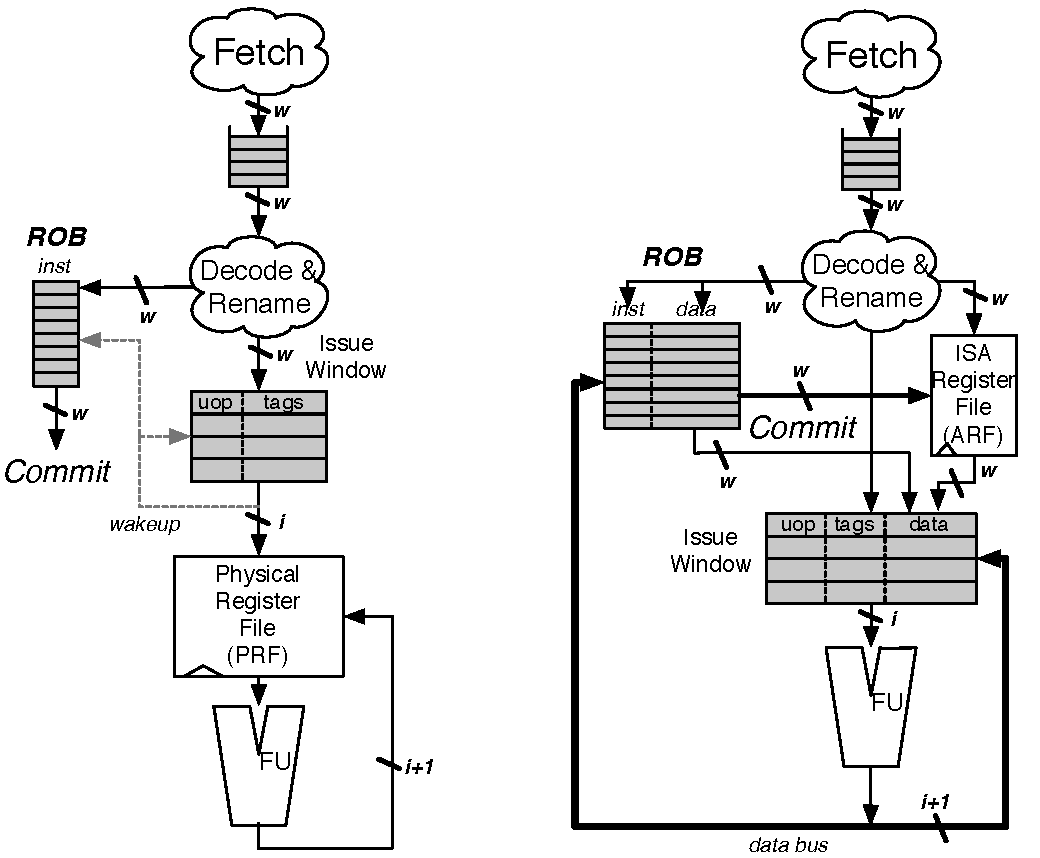
\includegraphics[scale =0.8] {figures/prf-and-arf}}
	\caption{ \small A PRF design (left) and a data-in-ROB design (right).}
	\label{fig:prf_design}
\end{figure}
%\TODO{redo drawing without the +1 to reduce confusion}


This is in contrast to an ``implicit renaming" or ``data-in-ROB" out-of-order core design.  The Architectural Register File (ARF) only holds the committed register state, while the ROB holds the speculative write-back data.  On commit, the ROB transfers the speculative data to the ARF. \footnote{The Pentium 4 and the ARM Cortex A57 are examples of {\em implicit renaming} designs.}




\begin{figure}[htb]
	\centering
	\centerline{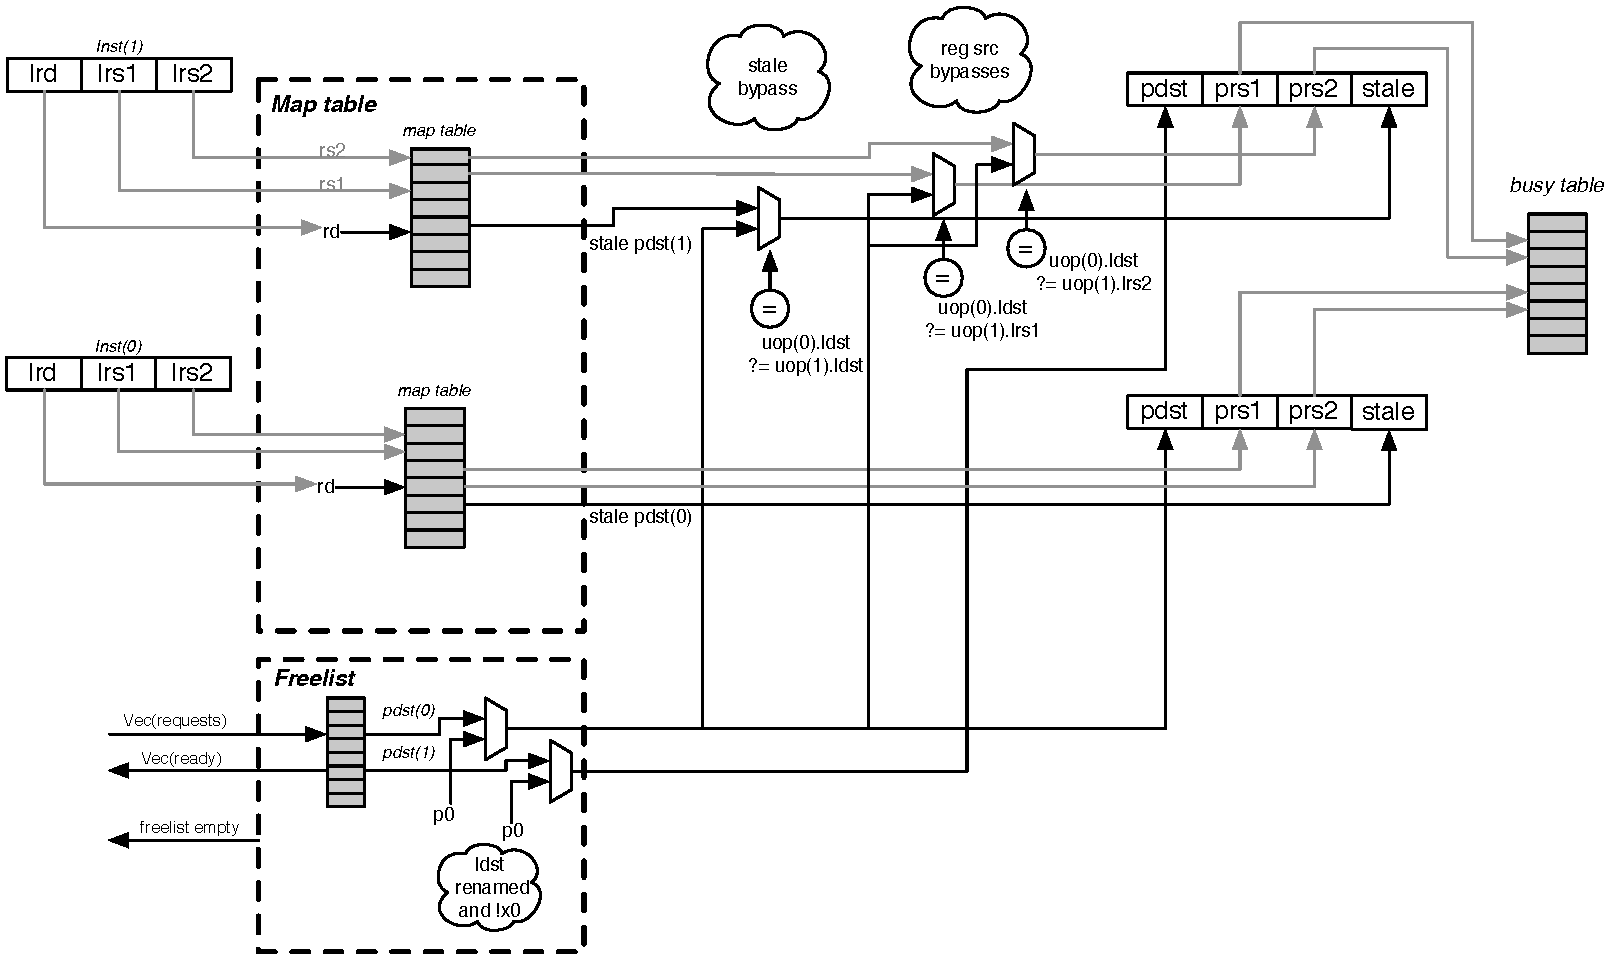
\includegraphics[scale =0.6] {figures/rename-pipeline}}
	\caption{ \small The Rename Stage. Logical register specifiers read the map table to get their physical specifier. For superscalar rename, any changes to the map tables must be bypassed to dependent instructions. The physical source specifiers can then read the Busy Table. The {\em Stale} specifier is used to track which physical register will be freed when the instruction later commits. P0 in the Physical Register File is always 0.}
	\label{fig:rename-pipeline}
\end{figure}
%TODO{remove lrd, and change to ldst?}


\section{The Rename Map Table}

The Rename Map Table holds the speculative mappings from ISA registers to physical registers.  

Each branch gets its own copy of the rename map table.\footnote{An alternate design for wider pipelines may prefer to only make up to one snapshot per cycle, but this comes with additional complexity to deduce the precise mappings for any given instruction within the fetch packet.}  On a branch mispredict, the map table can be reset instantly from the mispredicting branch's copy of the map table. 

As the RV64G ISA uses fixed locations of the register specifiers (and no implicit register specifiers), the map table can be read before the instruction is decoded!  

\subsection{Resets on Exceptions and Flushes}


An additional, optional ``Committed Map Table" holds the rename map for the committed architectural state.  If enabled, this allows single-cycle reset of the pipeline during flushes and exceptions (the current map table is reset to the committed map table). Otherwise, pipeline flushes require multiple cycles to ``unwind" the ROB to write back in the rename state at the commit point, one ROB row per cycle.


\section{The Busy Table}

The Busy Table tracks the readiness status of each physical register. If all physical operands are ready, the instruction will be ready to be issued. 

\section{The Free List}

The free-list tracks the physical registers that are currently un-used and is used to allocate new physical registers to instructions passing through the {\em Rename} stage.  

The Free List is implemented as a bit-vector.  A priority decoder can then be used to find the first free register. BOOM uses a cascading priority decoder to allocate multiple registers per cycle.\footnote{A two-wide rename stage could use two priority decoders starting from opposite ends.}

On every branch (or jalr), the rename map tables are snapshotted to allow single-cycle recovery on a branch misprediction. Likewise, the Free List also sets aside a new ``Allocation List", initialized to zero.  As new physical registers are allocated, the Allocation List for each branch is updated to track all of the physical registers that have been allocated after the branch. If a misspeculation occurs, its Allocation List is added back to the Free List by {\em OR'ing} the branch's Allocation List with the Free List.\footnote{Conceptually, branches are often described as ``snapshotting" the Free List (along with an {\em OR'ing} with the current Free List at the time of the misprediction). However, snapshotting fails to account for physical registers that were allocated when the snapshot occurs, then become freed, then becomes re-allocated before the branch mispredict is detected.  In this scenario, the physical register gets leaked, as neither the snapshot nor the current Free List know that it had been freed.  Eventually, the processor slows as it struggles to maintain enough inflight physical registers, until finally the machine comes to a halt. If this sounds autobiographical because the author may have trusted computer architecture lectures, well...}

\section{Stale Destination Specifiers}

For instructions that will write a register, the map table is read to get the {\em stale physical destination specifier} (``stale pdst").  Once the instruction commits, the {\em stale pdst} is returned to the free list, as no future instructions will read it.

%\section{Handling Branch Mispredictions}
%
%Every instruction in the pipeline has a ``branch mask", which is a bit-vector describing each live branch that it is currently being speculated under. Each branch is allocated a ``branch tag", and a corresponding branch mask bit such that every following instruction will have that corresponding bit set in its own branch mask.  Once a branch is resolved, the corresponding branch mask bit is cleared in every instruction's branch-mask. If the branch is misspeculated, then all instructions with the corresponding branch mask bit is killed. 



